\chapter{Theory}
\label{sec:theo}

%In diesem Kapitel beschreiben Sie Ihren eigenen Beitrag
%- Es muss klar sein, worin die eigentliche Innovation besteht#

\section{Quadcopter Modelling}

\todo{fundamental physics}

\todo{particle simulation}



\section{Vrep}

\todo{connecting visual representation and physical model}

\todo{simulation structure (lua scripts, scene structure}

\todo{lua module structure}

\todo{external interface (signals)}

\section{Communication V-REP-Quadrocopter}
\textbf{\textit{Goal}:} our mixed reality simulation needs a dependable link of communication between the V-REP simulation environment and the flying quadrocopters. The Quadcopter needs to stream its telemetry data in real-time to the V-REP, and the reverse communication is needed as well.\\
The simulated quadrocopters that we have in the V-REP are divided into two categories: real and virtual representations.\\ 
The real are replicating the physical flying quadrocopters. They should perform the same flying manoeuvres as those flying in the real environment. In order to make the model replicate this behaviour, the flying quadrocopter must send its linear and angular velocity, its pitch yaw and row and other parameters in real time to its representation model in V-REP. The simulation model should also send the readings from its proximity sensors to the flying quadcopter thus providing it with information from a virtual sensor. \\
The virtual quadrocopters are purely simulation quadcopter objects, that exist only in the V-REP simulation environment. Their purpose is to interact with the real quadrocopters for example to avoid collisions and thus making the first steps in the swarm research. The virtual quadrocopters have to be seen in the Paparazzi ground station as if they are real physical quadrocopters. It means that all the ground station agents like message logger, the signal plotting, attitude indicator, artificial horizon and other displays have to be updated with adequate information coming from the virtual quadrocopters in the V-REP.

The communication between the V-REP quadrocopter models and the physical quadrocopters passes through several software components, which are depicted on figure \ref{fig:communication} and discussed in the next chapters.

\begin{figure}[h!]
 \begin{center}
  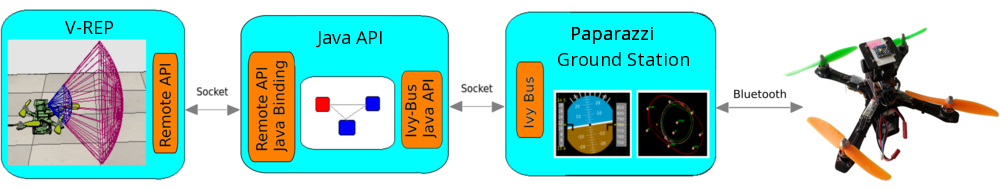
\includegraphics[scale=0.15]{communication.png}
 \end{center}
  \caption{communication V-REP - Quadrocopter\label{fig:communication}}
\end{figure}

\subsection{V-REP Remote API}
V-REP provides several means of communication with an external application. One of them is the Remote API, which allows to control a simulation (or the simulator itself) from an external application or a remote hardware (e.g. real robot, remote computer, etc.). The V-REP remote API is composed by approximately one hundred functions that can be called from a C/C++ application, a Python script, a Java application, a Matlab/Octave program, an Urbi script, or a Lua script. The remote API functions are interacting with V-REP via socket communication in a way that reduces lag and network load to a great extent.

\subsection{Java API}
Java API is the external program, that we have implemented to communicate with V-REP through the Remote API.
We have chosen to implement our external program, communicating with the V-REP, in the Java programming language regarding the following advantages: Java's platform independence allows to run the external program even on different machine with different operating system than the one used for running the V-REP environment.  Java is object-orientated which favours the use of design patterns and highly abstraction layers, which allows us to write an API that is modular, reusable and can later be easily extended to support other mixed-reality scenarious. The implementation and architecture of the Java API is duscussed in details in \ref{sec:implementation}. The purpose of the Java application is to serve as a communicating bridge between the Paparazzi Ground Station and the V-REP. It detects all quadrocopters in the V-REP simulation, builds their virtual representations and feeds the models with real-time data.

\subsection{Ivy Bus}
Ivy Bus is a simple protocol and a set of open-source (LGPL) libraries and programs that allows applications to broadcast information through text messages, with a subscription mechanism based on regular expressions. Ivy libraries are available in C, C++, Java, Python and Perl, on Windows and Unix boxes and on Macs. The Paparazzi Ground Station uses the Ivy Bus as a means of communication between the different software components. Figure \ref{fig:paparazziGS} depicts the communication structure in the Paparazzi Ground Station, in which the different agents communicate with each other by sending messages on the Ivy-Bus.

\begin{figure}[h!]
 \begin{center}
  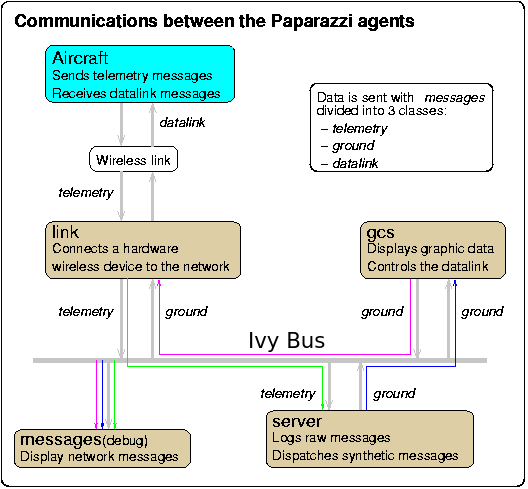
\includegraphics[scale=0.7]{paparazzi_gs.png}
 \end{center}
  \caption{Ivy-Bus in Paparazzi Ground Station\label{fig:paparazziGS}}
\end{figure}

The UAV (in blue) is streaming its telemetry data to the ground control station, which is received by the link. The \textbf{link} agent manages the ground-based radio modem and distributes the received messages to the other agents across the Ivy-Bus.

The Ivy Bus is an example of a publisher-subscriber protocol, in which senders of messages, called publishers, does not  explicitly specify the address of the receiver, but just send the message on one, shared by all nodes, bus. The recipients, called subscribers, which are interested in the message will accept it and the others will ignore it. The publisher-subscriber is a many to many communication model in which publishers are loosely coupled to subscribers - there is no space, flow and time coupling. This means that the publishers does not have to know the addresses of the subscribers and event does not need to know of their existence. Each can operate normally without the other and can continue its thread of execution regardless if the subscriber has received the message or not. It also provides scalability, which means that we can “attach” our Java API to the Ivy-Bus and start publishing and listening for messages without changing any line of source code in the Paparazzi Ground Station software.

In the publisher-subscriber model, subscribers typically receive only a subset of the total messages published. The process of selecting messages for reception and processing is called filtering. There are two common forms of filtering: topic-based and content-based.
In a topic-based system, messages are published to "topics" or named logical channels. Subscribers in a topic-based system will receive all messages published to the topics to which they subscribe, and all subscribers to a topic will receive the same messages. The publisher is responsible for defining the classes of messages to which subscribers can subscribe.
In a content-based system, messages are only delivered to a subscriber if the attributes or content of those messages match constraints defined by the subscriber. The subscriber is responsible for classifying the messages. Both filtering techniques are depicted in figures \ref{fig:pubsubsc_topic_based} and \ref{fig:pubsubsc_content_based}.

The Ivy Bus is a content-based publisher-subscriber and uses regular expressions for the message filtering.

\begin{figure}[!tbp]
  \centering
  \begin{minipage}[b]{0.4\textwidth}
    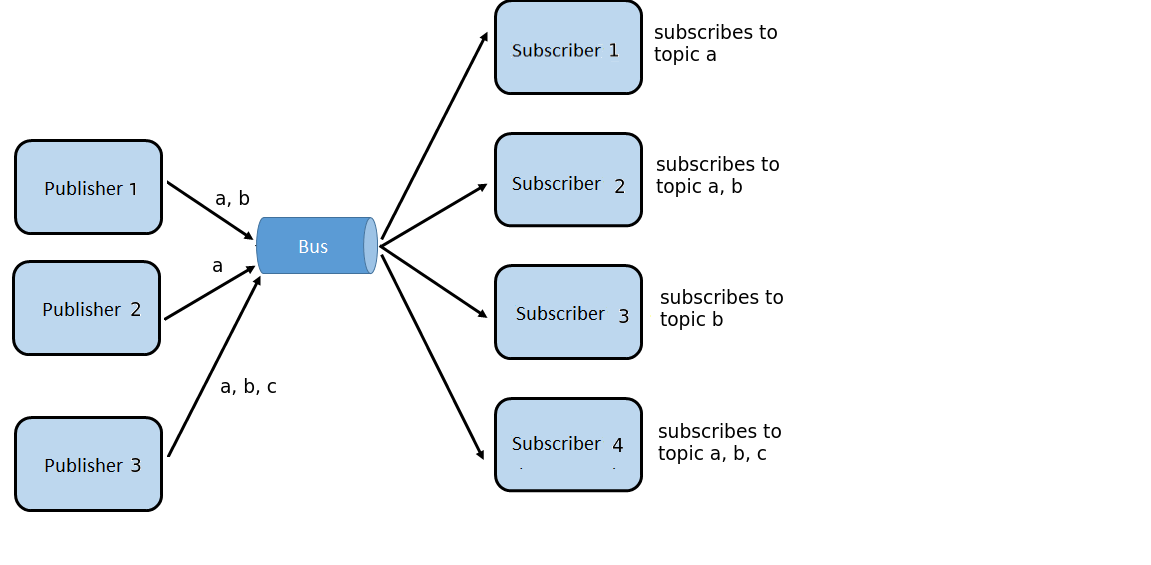
\includegraphics[scale=0.4]{pubsubsc_topic_based.png}
    \caption{Topic-based publisher-subscriber \label{fig:pubsubsc_content_based}}
  \end{minipage}
  \hfill
  \begin{minipage}[b]{0.4\textwidth}
    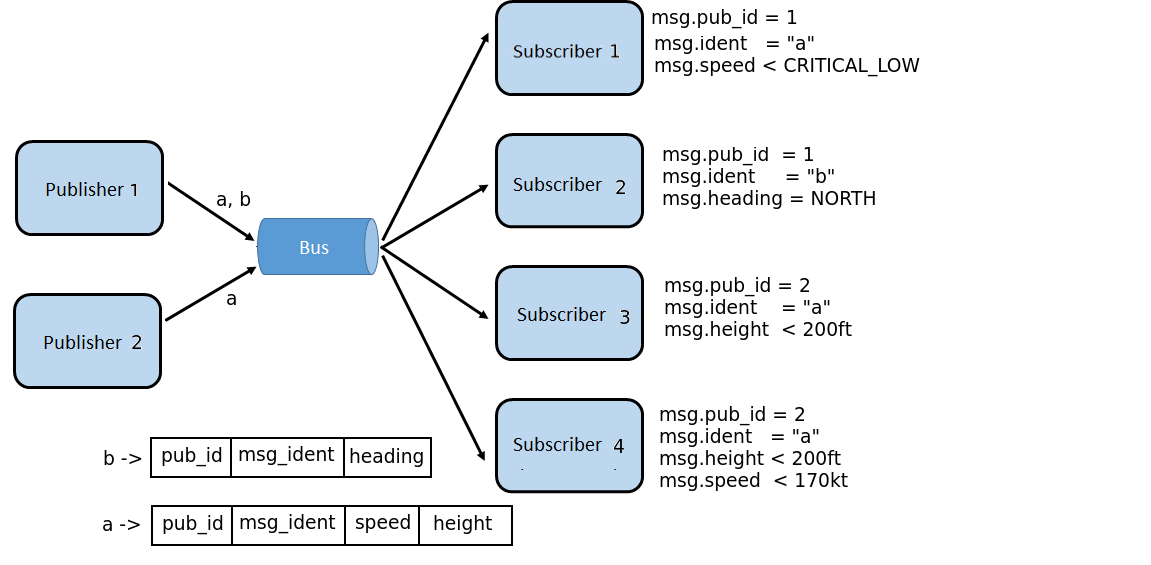
\includegraphics[scale=0.4]{pubsubsc_content_based.png}
    \caption{Content-based publisher-subscriber \label{fig:pubsubsc_topic_based}}
  \end{minipage}
\end{figure}

\subsection{Communication}

The communication between V-REP and the quadrocopters passes through the Java API, which serves as a bridge between them. In fact the Java API does not communicate directly with the quadrocopter, but connects to the Ivy-Bus in the Paparazzi GS and can thus subscribe to the messages caring the telemetry data and also publish messages which will eventually be send to the quadrocopter by the link agent.
Since we wanted to create a modular and reusable API, that can be used for other mixed-reality scenarios, the Java API was created with the idea in mind to be distributed, modular and rely on many abstraction layers. The API development has followed the specification-driven principles and its main tasks are described as follows:

\subsubsection{V-REP connection through Remote API}


% example for definition    
% \begin{definitionnonum}[Softwarearchitektur ]
% Die Softwarearchitektur repräsentiert alle Softwarekomponenten und deren Interaktionen in einer hierarchischen Struktur. Es werden sowohl statische Aspekte wie Schnittstellen und Datenpfade zwischen Softwarekomponenten, als auch dynamische Aspekte wie Prozessabläufe und zeitliches Verhalten beschrieben.
% \end{definitionnonum} 
 

  
%  example for bulletpoints
%\begin{itemize}    
%	\item{(überarbeiteter) Sicherheitsplan nach ISO 26262-6:2011, 5.5.1}
%	\item{Design- und Programmierrichtlinien für Programmier- und Modellierungssprachen nach ISO 26262-6:2011, 5.5.5}
%	\item{Hardware-Software-Interfacespezifikation nach ISO 26262-4:2011, 7.5.6}
%	\item{Software-Sicherheitsanforderungen nach ISO 26262-6:2011, 6.5.1}
%	\item{(überarbeiteter) Software-Verifizierungsplan nach  ISO 26262-6:2011, 6.5.3}
%	\item{Software-Verifizierungsbericht nach ISO 26262-6:2011, 6.5.4}
%\end{itemize}

 
%example for table    
% \begin{table}[h]
%      \centering
%    \caption{7.4.1 Notationen für Softwarearchitekturen\cite{iso6}}
%    \begin{tabular}{|c|l|c|c|c|c|}
%      \hline
%     \multicolumn{2}{|c|}{\multirow{2}{*}{Methoden}} & \multicolumn{4}{|c|}{ASIL}\\
%      \multicolumn{2}{|c|}{} &A & B & C & D\\
%      \hline
%       1a & Informelle Notationen & ++ & ++ & + & +\\
%      \hline
%       1b & Semi-formale Notationen & + & ++ & ++ & ++\\
%      \hline
%        1c & Formale Notationen & + & + & + & +\\
% 
%      \hline
%      \end{tabular}
%      \label{tab:archDescr}
%\end{table}
